\documentclass[10.5pt,a4paper]{article}
\usepackage[UTF8]{ctex}
\usepackage{tikz}  
\usepackage{amsmath}
\usepackage{amsfonts}
\usepackage{amssymb}
\usepackage{graphicx}
\usepackage{algorithm2e}
\usepackage{listings}
\usepackage{float}
\usepackage[top=10mm, bottom=12.5mm, left=12.5mm, right=12.5mm]{geometry}
\makeatletter
\renewcommand{\@makecaption}[2]{%
\vspace{\abovecaptionskip}%
\sbox{\@tempboxa}{#1. #2}
\ifdim \wd\@tempboxa >\hsize
#1. #2\par
\else
\global\@minipagefalse
\hbox to \hsize {\hfil #1. #2\hfil}%
\fi
\vspace{\belowcaptionskip}}
\makeatother
\lstset{
  basicstyle=\small,
  numbers=left,
  keywordstyle=\color{blue},
  numberstyle={\tiny\color{lightgray}},
  stepnumber=1, %行号会逐行往上递增
  numbersep=5pt,
  commentstyle=\small\color{red},
  backgroundcolor=\color[rgb]{1,1,1},
  showspaces=false,
  showtabs=false,
  frame=shadowbox, framexleftmargin=5mm, rulesepcolor=\color{red!20!green!20!blue!20!},
% frame=single,
%  TABframe=single,
  tabsize=4,
  breaklines=tr,
  extendedchars=false %这一条命令可以解决代码跨页时,章节标题,页眉等汉字不显示的问题
}
\usepackage{titlesec}
%\titlelabel{\thetitle.\quad}
\titleformat{\section}
  {\normalfont\fontsize{10.5}{15}\bfseries}{\thesection.\quad}{0.5em}{}
\titleformat{\subsection}
  {\normalfont\fontsize{10.5}{15}\bfseries}{\thesubsection}{1em}{}
%\renewcommand{\thesection}{\arabic{section}.}
\date{}
\title{Simulated Annealing-The Implementation and Performance Analysis} 
\author{Luezhen Yuan(袁略真)\footnote{Student ID: 3130103964. Major: Bioinformatics. Email: 3130103964@zju.edu.cn}}
\begin{document}
\maketitle
\section*{}
\paragraph{Abstract:}Simulated annealing is a metaheuristic algorithm used to solve combinatorial optimization problem. However, the choose of annealing schedule is not discussed in many textbooks. This article implement the simulated annealing algorithm in C++ in a generic style, and test the program on the Traveling Salesman Problem(TSP) for 4 annealing plans and each one runs 10 configurations. The results show that a slow temperature decreasing plan is likely to find a good optimization solution, however the time cost is too big. Setting the $r=$0.99999 and running 10 configurations can give a good solution and the time cost is affordable.

\paragraph{Keywords:}Simulated Annealing; Annealing schedule; Combinatorial optimization; Traveling salesman problem; Generic programming; Object-oriented programming

\section{Introduction}
The simulated annealing is a metaheuristic method to find the global minimum of a combinatorial optimization problem\cite{3}. The problem is often an NP-complete problem, which means finding the exact solution will cost polynomial time. This method is a Markov Chain Monte Carlo(MCMC) based method, and allows worse solutions in the Markov Chain. The method is also featured by its use of the decreasing temperature, which is an efficient improvement of the Metropolis procedure.


The simulated annealing is introduced by S. Kirkpatrick\cite{1} in 1983. The most procedure in the simulated annealing algorithm is the same as Metropolis's algorithm, but the use of deceasing temperature. Metropolis's algorithm is a Markov chain Monte Carlo sampling method that used for simulation used in statistical mechanics. The simulated annealing, however, is an heuristic method used to solve combinatorial optimization problem.

This article implements the simulated annealing in C++ in a generic style. The generic programming is an efficient method to separate algorithms from data structures. In C++, these methodology is characterized by the use of parametric polymorphism through the use of templates. In the generic programming, an important term is the \textit{concept}, which is a set of requirements that describe the interface and semantic behaviour of an unknown data structure used in a generic algorithm. This article use a abstract base class to store the concept.

\section{Simulated Annealing and Implementation}

\subsection{Procedure in Simulated Annealing}
The simulated annealing method simulate the annealing procedure, which starts from a high temperature, and then slowly decreases the temperature of a system. The slowly decreasing temperature is a central feature of the method. When the temperature is high, the system can almost free from changing to the other states. As the temperature decrease, it's more likely to change to a lower energy state than climb up the energy mountain. Climbing up is valuable for jumping out of a local minimum valley. When the temperature is decreased closely to zero, the system is reluctant from climbing up the mountain. And now, the state is likely to be a global minimum.
\subsection{Terms in Simulated annealing}
The simulated annealing is a Markov Chain Monte Carlo(MCMC) method, and many terms mentioned following are the same as other MCMC.

The simulated annealing procedure is a Markov Chain because the \textit{neighbours of a state} and the \textit{transition probability} only depend on the state. The neighbours of a current state is a subset of all possible states which can be \textit{move}d to from the current state. These moves usually defined under simple rules, and can be seen as \textit{a small random displacement}.

The states of a system can be described quantitatively using the \textit{energy}. The energy, in the optimization problem, is the target function that you want to minimize. Two states can be compared using the Boltzmann probability factor, $\pi(s)=exp(-E(s)/k_BT)$\cite{1}, where \textit{s} is a state of the system, and $E(s)$ is the energy of this state. Under the condition of the existence of stationary distribution in Markov Chain, the transition probability should follows, $\pi(s)P(s\rightarrow s') = \pi(s')P(s'\rightarrow s)$. Metropolis choose the following transition probability:
\begin{equation}
P(s\rightarrow s')=\left\lbrace 
\begin{aligned}
&e^{-\Delta E/k_BT}&,\ \Delta E>0\\
&1&,\ \Delta E\leqslant 0
\end{aligned}\right. 
\end{equation}

The terms mentioned above, actually, is the Metropolis algorithm. The feature of the simulated annealing algorithm, which different from the Metropolis's one, is the decreasing temperature. An \textit{annealing schedule} is a predefined rule that quantify how the temperature will decrease. For example, $T(t_{n+1})=rT(t_n)$, where \textit{n} is the simulation time step, \textit{T} is the temperature at that step, \textit{r} quantify how fast the temperature will decrease.
\subsection{Implementation Using the Generic Programming Method}
\begin{algorithm}[H]
\KwIn{$start\_state,\ max\_iteration,\ r$}
\KwOut{$fineal\_state$}
$temperature \gets 100$\;
$state \gets start\_state$\;
\For{$t \gets 0$ \KwTo $max\_iteration$}{
	$energy_1 \gets$ current $stage$ energy\;
	$state\_tmp \gets$ a neighbour of the $state$\;
	$energy_2 \gets$ $stage\_tmp$ energy\;
	$transition\_probability \gets e^{-\Delta E/k_BT}$\;
	$p \gets$random number generator[0,1)\;
	\If{$p<transition\_probability$}{
		$state \gets state\_tmp$\;
	}
	\Else{
		drop $state\_tmp$\;
	}
	$temperature \gets temperature*r$\;
}
return $state$\;
\caption{Simulated Annealing Algorithm}
\end{algorithm}

To implement a generic simulated annealing algorithm, I design the header of the template function $Simulated\_Annealing$:
\begin{lstlisting}[language=c++]
template <class State>
State Simulated_Annealing(Simulated_Annealing_Problem<State>* pSAP,int iteration=100000,double downratio=0.999, string file_name="Simulated_Path.txt",void m_free(State pst)=my_free, double m_next(double current_temperature,double downratio)=my_next,double Acceptance(Simulated_Annealing_Problem<State>* pSAP,State st1, State st2, double temperature)=my_Acceptance );
\end{lstlisting}
Here, the $Simulated\_Annealing\_Problem$ is an abstract base class, storing the concept asked in the template function $Simulated\_Annealing$. The concept is some member functions used in the generic algorithm.
\begin{lstlisting}[language=c++]
class Simulated_Annealing_Problem{
public:
virtual State initial_state()=0;
virtual double energy(State state)=0;//[0 1]
virtual State neighbour(State state)=0;
};
\end{lstlisting}
\section{Test Performance on the Traveling Salesman Problem(TSP)}
\subsection{Introduction to the TSP}
The TSP is a combinatorial optimization problem, and also belongs to the class of NP-complete problem, which need polynomial time to find the exact solution. TSP tells this story: A salesman want to find a shortest route to travel N given cities.
\subsection{Derived Class for TSP}
To solve the TSP using the generic simulated annealing algorithm, I design a derived class of the $Simulated\_Annealing\_$ $Problem$(an abstract base class, mentioned in the previous section.) for TSP.


\begin{lstlisting}[language=c++]
class TSP:public Simulated_Annealing_Problem<int*>{
double* m_distance;
double max_length;
public:
int m_size;
TSP(string data_file="TSPdata.txt");//Input file. The coordinate of each city.
int* initial_state();
double energy(int* state);//[0 1]
int* neighbour(int* state);
double& distance(int i, int j);//A[i][j]=distance[(2*m_size-i)(i-1)/2+j-i];
};
\end{lstlisting}
\subsection{Test Cases and Results}
Figure \ref{fig:4} shows the simulated annealing procedure under $r=$0.999.
\begin{figure}[H]
\centering
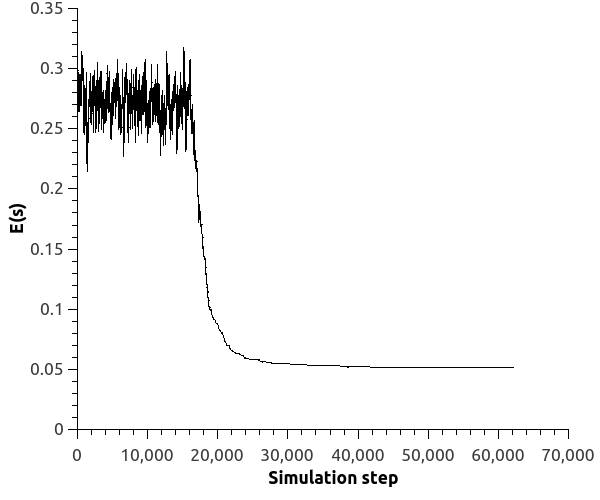
\includegraphics[width=0.6\textwidth]{../result/SA_1_1_procedure.png}
\caption{Common simulated annealing procedure. The simulation is performed under $r=$0.999.}
\label{fig:4}
\end{figure}

To test the performance of the generic algorithm and study the annealing schedule, I change the value of the important parameter $r$. Let $r$=0.999,0.9999,0.99999, and 0.999999. Each runs 10 configurations(10 times). The figure \ref{fig:1},\ref{fig:2}, and \ref{fig:3} shows the results. The data of 100 cities and one starting city comes from \cite{4}.

Figure \ref{fig:1} shows the best solution for each $r$ in 10 configurations. Figure \ref{fig:2} shows the solution distribution on on each $r$. Figure \ref{fig:3} shows the time cost on each $r$. The time cost is related to the iteration times in one run. However, when the system is trapped in a state for a long time(20\% of the $iteration$), the iteration will stop, even if the max iteration time(here $iteration$) isn't reached. Here, the iteration time in one run is calculated by the simple formula(100 is the start temperature.):
$$t_{low}=100*r^{iteration}$$
$$iteration=\frac{log(t_{low}/100)}{log(r)}$$
To compare the time costs on each configurations, I set the $t_{low}=10^{-25}$.

\begin{figure}[H]
\begin{minipage}[b]{0.5\linewidth}
\centering
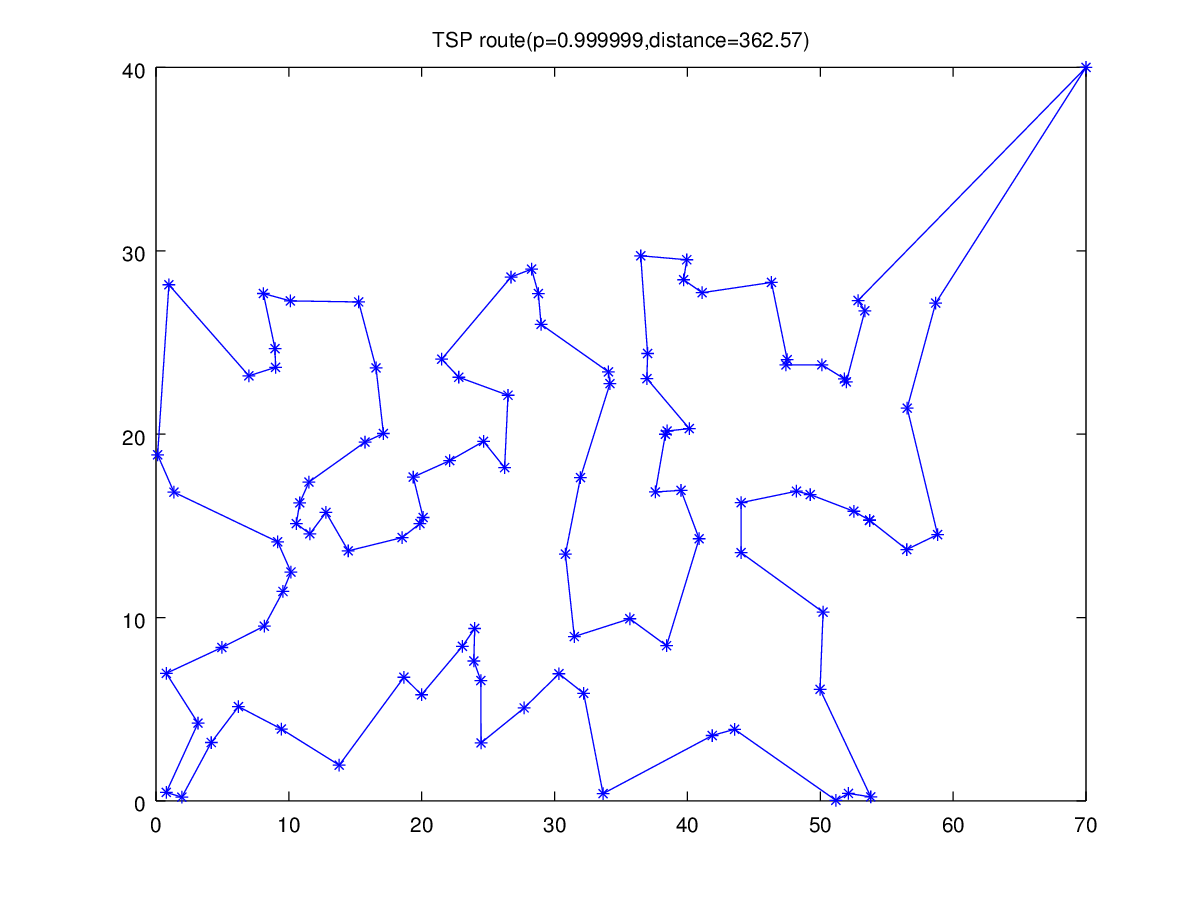
\includegraphics[width=\textwidth]{../result/TSP_route_362.png}
\end{minipage}
\hspace{0.5cm}
\begin{minipage}[b]{0.5\linewidth}
\centering
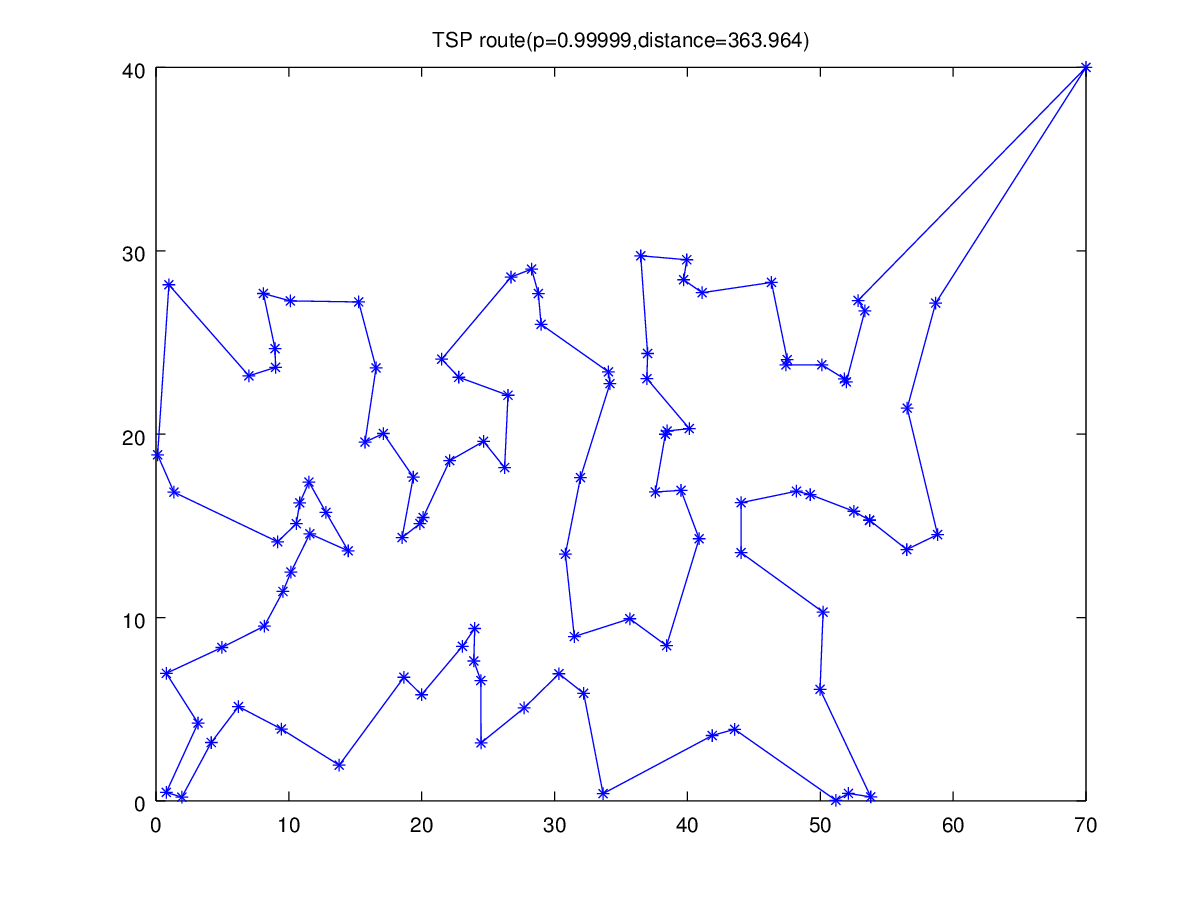
\includegraphics[width=\textwidth]{../result/TSP_route_363.png}
\end{minipage}
\begin{minipage}[b]{0.5\linewidth}
\centering
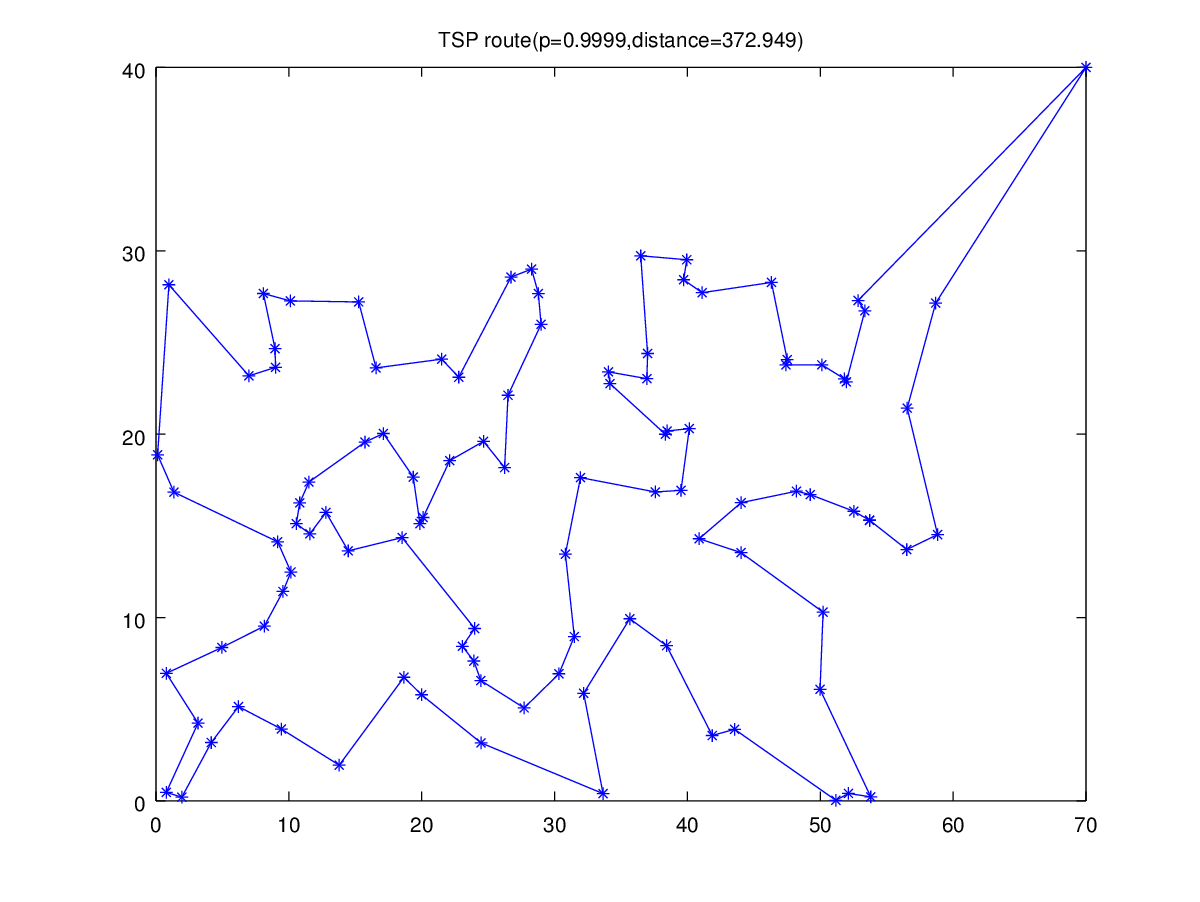
\includegraphics[width=\textwidth]{../result/TSP_route_372.png}
\end{minipage}
\hspace{0.5cm}
\begin{minipage}[b]{0.5\linewidth}
\centering
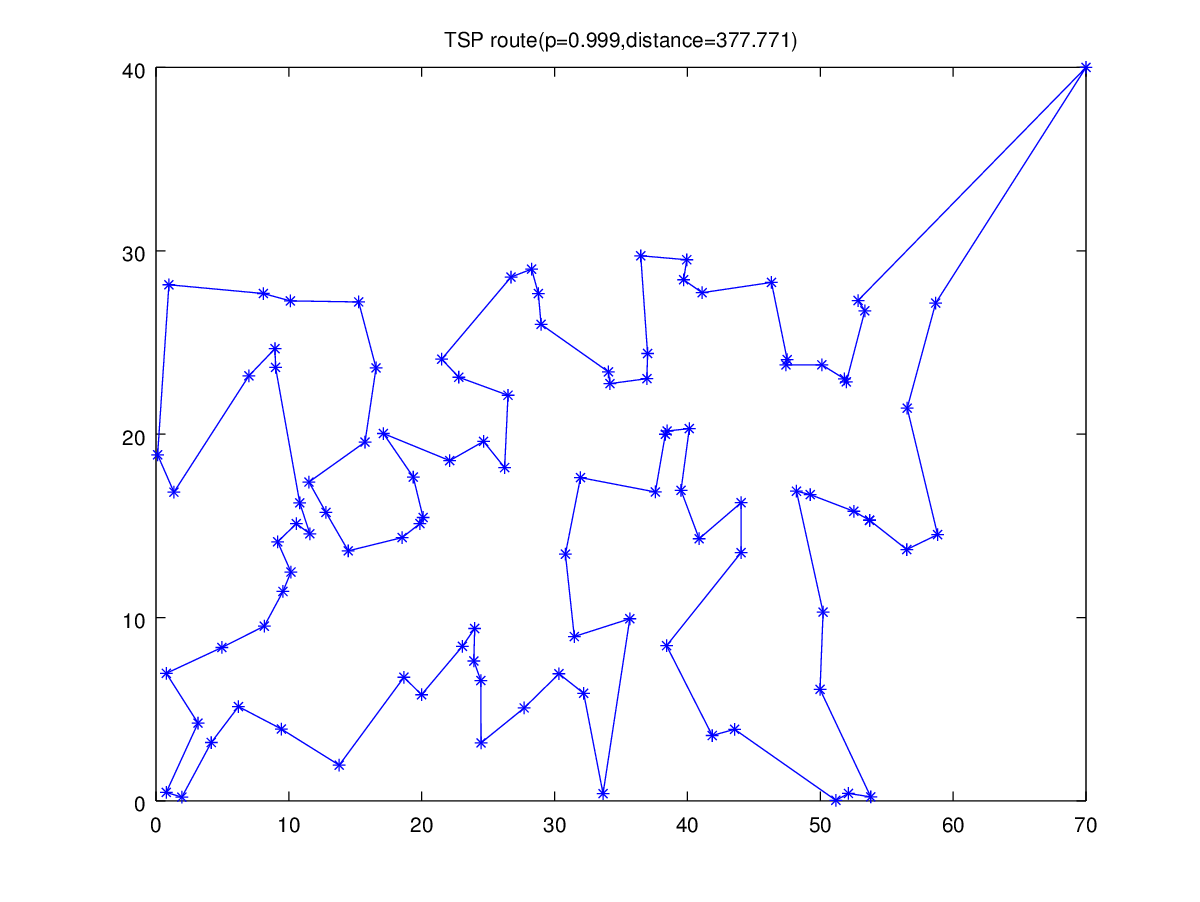
\includegraphics[width=\textwidth]{../result/TSP_route_377.png}
\end{minipage}
\caption{TSP routes on four $r$s. Top left: $r$=0.999999, distance=362.57; Top right: $r$=0.99999, distance=363.964; Bottom left: $r$=0.9999, distance=372.949; $r$=0.999, distance=377.771;}
\label{fig:1}
\end{figure}


\begin{figure}[H]
\begin{minipage}[b]{0.5\linewidth}
\centering
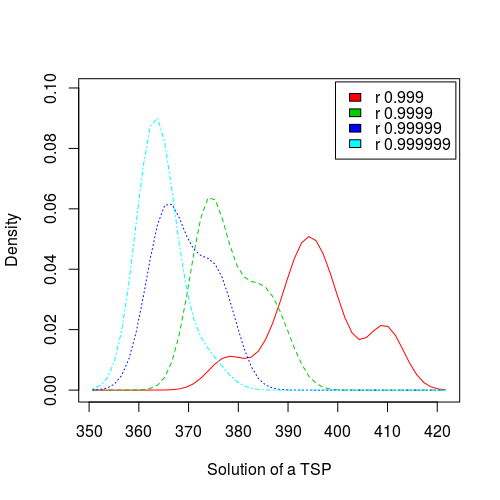
\includegraphics[width=\textwidth]{../result/SAonDiffPlan3.png}
\caption{SA performance on finding the optimization.}
\label{fig:2}
\end{minipage}
\hspace{0.5cm}
\begin{minipage}[b]{0.5\linewidth}
\centering
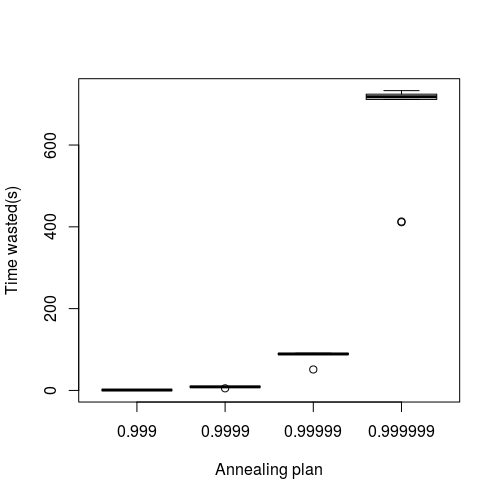
\includegraphics[width=\textwidth]{../result/SAonDiffPlanTime3.png}
\caption{SA performance on finding the optimization.}
\label{fig:3}
\end{minipage}
\end{figure}

Figure \ref{fig:2} shows that with the r increase(the decrease of temperature slower), the solution distribution shift left. Figure \ref{fig:3} shows that with the r increase, the time cost grows extremely fast.
\section{Discussions and Conclusions}
The simulated annealing is a useful method for wide spread problems. In \cite{book,3}, they conclude that if a problem follows the following conditions, they can be solved using the method:
\begin{enumerate}
\item Solution can be quantified by number.(Here, the energy function.)
\item An initial solution can be easily computed.(For example, generate a TSP route randomly)
\item There are simple adjustment rules that locally change a solution.(The solution means the state of a system.)
\item Every solution can be turned into every other solution by the adjustment rules.
\item Often used when the search space is discrete.
\end{enumerate}

However, to solve these problems, we should set same parameters in the algorithm. From figure \ref{fig:2} and \ref{fig:3}, the paradox of $r$ appears. High $r$ is good for finding the optimization solution, however the time cost is too big to afford. If we set $r$=0.99999, the time cost is around 150(s), however the solution distribution is not a single peak, which means we should run many configurations and find the best solution. Figure \ref{fig:1} top right shows that choosing $r$=0.99999 and run 10 configurations is likely to appear a good solution. If we set $r=$0.9999 or 0.999, even if we run many configurations, the solution is not good(See figure \ref{fig:1} bottom panel, and figure \ref{fig:2}).

In conclusion, $r$=0.99999 and running 10 configurations is a good choice of the simulated annealing method, and the time cost is affordable..


\section{Acknowledgement}
Prof. Yizhi Tan(谈之奕)(School of Mathematical Sciences) is the course director of \textit{Applied Operational Research(应用运筹学)} in Zhejiang University, Hangzhou, China. In the course, I learnt linear programming, integer programming, graph theory, combinatorial optimization(NP-complete problem, TSP, and so on), scheduling, and game theory. In computational biology, bioinformatics, and computational systems biology, there are some problems that have been solving using the methods mentioned in this course. In metabolic network analysis, the flux balance analysis is a linear programming problem. In molecular phylogeny, the branch-and-bound method also used in constructing some phylogenetic trees.  Thanks to Prof. Yizhi Tan.

Prof. Dafang Zheng(郑大昉)(Department of Physics) is the course director of \textit{Computational Physics(计算物理学)} in Zhejiang University, Hangzhou, China. The Monte Carlo simulation, Metropolis Markov Chain Monte Carlo Simulation is lectured in this course. Thanks to Prof. Dafang Zheng.


\section{Supplement}
The source code, this document, the figures, and program's output data are accessible in.
\section*{}
\begin{thebibliography}{ieee}
\bibitem{1}S. Kirkpatrick, C. D. Gelatt, and M. P. Vecchi, “Optimization by Simulated Annealing,” Science, vol. 220, no. 4598, pp. 671–680, May 1983.
\bibitem{book}B. Vöcking, H. Alt, M. Dietzfelbinger, R. Reischuk, C. Scheideler, H. Vollmer, and D. Wagner, Eds., Algorithms Unplugged. Berlin, Heidelberg: Springer Berlin Heidelberg, 2011.
\bibitem{3}Simulated annealing, Wikipedia, the free encyclopedia. 07-Apr-2016.
\bibitem{4}司守奎, 数学建模算法与应用. 北京: 国防工业出版社, 2011.
\end{thebibliography}
\end{document}